  \documentclass[crop,tikz]{standalone}% 'crop' is the default for v1.0, before it was 'preview'
%\usetikzlibrary{...}% tikz package already loaded by 'tikz' option
\usepackage[utf8]{inputenc}

\usepackage{tikz}
\usetikzlibrary{
  arrows,
automata,
backgrounds,
calc,
decorations.pathreplacing,
fit,
petri,
positioning,
shadows,
shapes,
snakes,
}


\begin{document}


  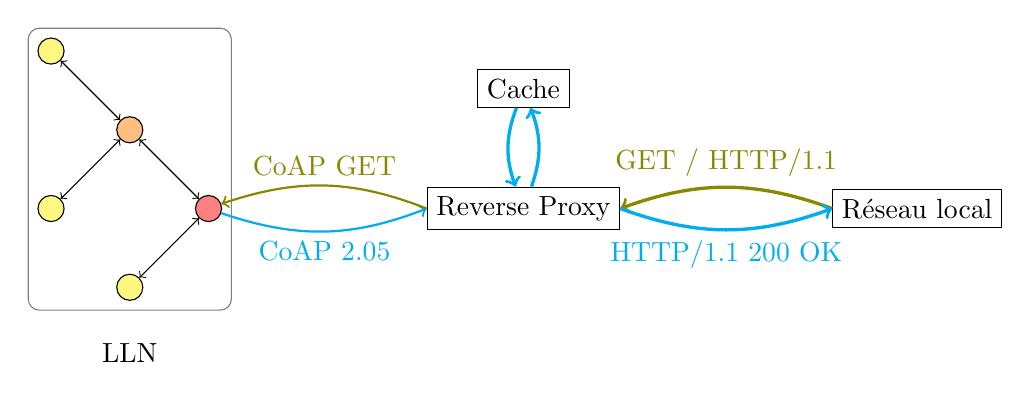
\begin{tikzpicture}

  % définition des styles
  \tikzstyle{visible}=[draw, fill=blue!50]
  \tikzstyle{hidden}=[ draw, fill=gray!20]
  \tikzstyle{router}=[circle, draw, fill=orange!50,text=black]
  \tikzstyle{child}=[circle, draw, fill=yellow!50,text=black]
  \tikzstyle{root}=[circle, draw, fill=red!50,text=black]

  % les nœuds
  \node[draw] (gw) {Reverse Proxy};

  \node[draw, above= of gw] (cache) {Cache};


  % Réseau contraint
  \node[root] (1) at (-4, 0) {};
  \node[router] (2) at (-5, 1) {};
  \node[child] (3) at (-5, -1) {};
  \node[child] (4) at (-6, 2) {};
  \node[child] (5) at (-6, 0) {};

  % \node[cloud, cloud puffs = 10, minimum width = 4cm, draw, fill = gray!10] (cloud) at (5,0) {Réseau local};
  \node[draw] (cloud) at (5,0) {Réseau local};

 \node [fit=(1) (2) (3) (4) (5), rounded corners, draw=black!50] (lln) {};
 \node [below=.3 cm of lln] {LLN};

\path

  % Réseau contraint
  (gw.west) edge[<-, cyan, thick, bend left=20] node [below] {CoAP 2.05} (1)
  (gw.west) edge[->, olive, thick, bend right=20] node [above] {CoAP GET} (1)
  (1) edge[<->] (2)
  (1) edge[<->] (3)
  (2) edge[<->] (4)
  (2) edge[<->] (5)

  (cache) edge[->, very thick, cyan, bend right=20] (gw)
  (cache) edge[<-, very thick, cyan, bend left=20] (gw)

  % Réseau conventionnel
  (gw.east) edge[<-, olive, very thick, bend left=20] node [above] {GET / HTTP/1.1} (cloud.west)
  (gw.east) edge[->, cyan, very thick, bend right=20] node [below] {HTTP/1.1 200 OK} (cloud.west)
  ;

  \end{tikzpicture}
\end{document}